\documentclass[a4paper, 14pt]{extarticle}
\usepackage{indentfirst}
\usepackage[T2A]{fontenc}
\usepackage[utf8]{inputenc}
\usepackage[english, russian]{babel}
\usepackage{amsmath, amssymb, amsthm, amscd, latexsym}
\usepackage[nottoc,numbib]{tocbibind}
\usepackage{graphicx, caption}
\usepackage[left=3cm,right=2cm,top=2cm,bottom=3cm]{geometry}
\setlength{\parindent}{1.25cm}
\linespread{1.25}
\graphicspath{{pictures/}}

\newtheorem{theorem}{Теорема}[subsection]
%\numberwithin{theorem}{subsection}
\newtheorem{lemma}{Лемма}
\newtheorem{corollary}{Следствие}
\newtheorem{proposition}{Предложение}
\newtheorem{assertion}{Утверждение}
\theoremstyle{definition}
\newtheorem{definition}{Определение}[subsection]
%\numberwithin{definition}{subsection}
\newtheorem{remark}{Замечание}
\newtheorem{example}{Пример}
\renewcommand{\thetheorem}{\arabic{theorem}}
\renewcommand{\thedefinition}{\arabic{definition}}

\usepackage{hyperref}
\hypersetup{
    colorlinks=true,
    linkcolor=blue,
    filecolor=magenta,      
    urlcolor=cyan,
    pdfpagemode=FullScreen,
}


\title{Проблема выразимости бинарных нейронных сетей}
\author{Р.\,С.~Мурадасилов}
\date{2020}

\begin{document}
\begin{titlepage}
\begin{center}
        
\textbf{Филиал Московского Государственного Университета\\
имени М.В. Ломоносова в г. Ташкенте} \vskip 0.3cm
\textbf{Факультет прикладной математики и информатики} \vskip 0.3cm
\textbf{Кафедра прикладной математики и информатики} \vskip 3cm
            
\textbf{Мурадасилов Руслан Серверович} \vskip 1cm
            
\textbf{КУРСОВАЯ РАБОТА} \vskip 1cm
            
\normalsize { \textbf{на тему: \guillemotleft Проблема выразимости бинарных нейронных сетей\guillemotright \\ \vskip 0.5cm
по направлению 01.03.02 \guillemotleft Прикладная математика и информатика\guillemotright} }
\vskip 1.5cm
\end{center}

\begin{flushleft}
Курсовая работа рассмотрена и рекомендована к защите \vskip 5pt
зав.кафедрой <<ПМиИ>>, д.ф.-м.н., профессор \rule{2.365cm}{0.5pt} Кудрявцев В.\,Б.
\end{flushleft}
\begin{flushleft}
Научный руководитель:\vskip 5pt
к.ф.-м.н. \rule{10.798cm}{0.5pt} Иванов И.\,Е.
\end{flushleft}
          
\begin{flushright}
<<\rule{1cm}{0.5pt}>>\rule{3.5cm}{0.5pt} 2020 г.
\end{flushright}
        
\vfill   
\begin{center}
Ташкент 2020
\end{center}
\end{titlepage}

\begin{abstract}
    В данной работе рассматривается проблема выразимости бинарной нейронной сети. Рассматривается проблема полноты класса бинарных нейронных сетей, слоем которой является композиция линейной булевой функции и нелинейного бинарного оператора. Исследуется вопрос глубины таких нейронных сетей для разных нелинейностей, что впоследствии может быть применено на практике. Обозначена проблема аппроксимации булевых функций линейными булевыми функциями и предложена идея доказательства того, что все нелинейные булевы функции достаточно далеки от линейных.
\end{abstract}

%\selectlanguage{english}

%\begin{abstract}
%    In this work
%\end{abstract}

%\selectlanguage{russian}

\setcounter{page}{2}
\newpage

\tableofcontents
\newpage

\section{Введение}
    За последнее десятилетие сложность и способности нейронных сетей существенно выросли, однако их потенциал до сих пор ограничивают стоимость и энергия потребления. Как известно, нейронные сети состоят из нескольких слоев взвешенных сумм, которые предсказывают нужный результат. Хранение всех значений чисел с плавающей запятой значительно увеличивает время обучения и требует большое количество памяти, что вызывает необходимость использовать только специальное оборудование, которое выдержит подобную нагрузку.
    
    Чтобы устройство с ограниченными ресурсами могло решать такие проблемы глубокого обучения, как распознавание лиц в реальном времени, необходимо использовать в качестве весов бинарные числа, а в качестве функций активации "--- бинарные аналоги функций активации в непрерывном случае, то есть <<бинаризовать>> нейронную сеть. Это позволит хранить гораздо больший объем данных, используя, например, 32-битный контроллер. Использование битовых операций сокращает время исполнения. Размеры бинарных нейронных сетей намного меньше, чем у их вещественнных аналогов. Точность моделей также меньше, но эта разница в точности постепенно сокращается и бинарные нейронный сети становятся точнее на больших датасетах, как ImageNet.
    
    В данной работе рассматривается вопрос полноты бинарной нейронной сети, то есть способность в точности выразить булеву функцию. А также ставится задача аппроксимации булевых функций, то есть способность выразить булеву функцию с некоторой допустимой погрешностью. С практической точки зрения устраивают оба варианта.
\newpage

\section{Историческая часть вопроса}
    Идея бинарной нейронной сети была впервые предложена Matthieu Courbariaux, где веса и функции активации используют только бинарные числа как и в обучении, так и в алгоритме обратного распространения ошибки с использованием метода градиентого спуска (SGD) \cite{first}.
    
    Чуть позже Mohammad Rastegari в модели XNOR-Net \cite{second} добавляет скалярное значение, чтобы компенсировать потерю информации во время бинаризации, который был получен из статистики весов и функций активации до бинаризации. Это улучшило общие показатели, но подсчет этого скалярного значения оказался дорогостоящим.
    
    Victor Zhou попытался обобщить квантизацию и использовал преимущество битовых операций для фиксированной точки данных, варьируя ее размерность \cite{third}. Zhou представил DoReFa-Net, модель с переменной размерностью весов, функций активации и даже вычисления градиента во время обратного распространения ошибки со значительно улучшенным временем обучения.
    
    Другие модели также добились положительных результатов. Zheng Tang ускорил время обучения, изучив как влияет скорость обучения на показатели нейронной сети и на колеблемость бинарных значений \cite{fourth}. Идея BNN+, созданная Sajad Darabi,также улучшает скорость обучения, использую другую эффективную функцию обратного распространения вместо импульсной \cite{fifth}.
    
    Сравнение результатов всех этих моделей на разных датасетах были подробно описаны в работе Taylor Simons и Dah-Jye Lee \cite{sixth}. Наглядно видно, что на MNIST, SVHN, CIFAR и ImageNet датасетах бинарные нейронные сети практически не уступают своим вещественнным аналогам.
\newpage

\section{Основные результаты}
\subsection{Полнота}
    Введем основные определения.
    \begin{definition}
    \emph{Бинарным оператором} называется конечный вектор $\overline{f} = (f_1, ..., f_n)$, в котором каждая $f_j$ является функцией алгебры логики от n переменных $(j = \overline{1, n})$.
    \end{definition}
    
    \begin{definition}
    Бинарный оператор называется \emph{линейным}, если каждая его компонента является линейной. Соответсвенно, бинарный оператор называется \emph{нелинейным}, если хотя бы одна из его компонент является нелинейной.
    \end{definition}
    
    \begin{definition}
    \emph{Слоем} называется композиция линейной булевой функции  и нелинейного бинарного оператора. \emph{Входным слоем} будем называть вектор $\overline{X} = (x_1, ... x_n)\in \{0, 1\}^n$, а \emph{выходным} "--- вектор $\overline{Y} = (y_1, ... y_m)\in \{0, 1\}^m$.
    Линейную часть слоя назовем \emph{весовой функцией}. Она применяется ко всем выходам предыдущего слоя, включая входной слой.
    Нелинейный оператор назовем \emph{функцией активации}. В качестве нее можно использовать и тождественный оператор.
    \end{definition}
    
    \begin{definition}
    \emph{Нейронной сетью} называется композиция функций, каждая из которых является слоем.
    \end{definition}
    
    Обозначим класс бинарных нейронных сетей с линейной булевой весовой функцией и нелинейным бинарным оператором в роли функции активации через $\mathfrak{B}$. Параметром этого класса будет семейство функций активации $F$. Справедлив следующий результат, относящийся к проблеме полноты бинарной нейронной сети с такой архитектурой.
    
    \begin{theorem}
    Какое бы семейство функций активации $F$ мы не взяли, класс бинарных нейронных сетей $\mathfrak{B}$ будет полон в $P_2$.
    \end{theorem}
    \begin{proof}
    Так как класс булевых линейных функций является предполным, то достаточно хотя бы одной нелинейной функции, чтобы нейронная сеть могла порождать $P_2$. По определению нелинейного бинарного оператора такая функция будет существовать, что доказывает теорему.
    \end{proof}
    
    Рассмотрим вопрос существования полной бинарной нейросети с двумя слоями. Справедлива следующая теорема.
    
    \begin{theorem}
    Существует бинарная нейронная сеть класса $\mathfrak{B}$ с двумя слоями, которая полна в $P_2$.
    \end{theorem}
    
    \begin{proof}
    Построим бинарную нейронную сеть, реализующую СДНФ функции. Во входном слое подаётся вектор $\overline{X} = (x_1, ... x_n)\in \{0, 1\}^n$, на котором хотим получить вектор значений. В первом слое будет бинарный оператор, состоящий из конъюнкций, то есть $f^1 = (f^1_1, ..., f^1_{2^n})$ $\forall f^1_j = \wedge$, $j = \overline{1, 2^n}$. Весовая функция $g$ первого слоя следующего вида: 
    \begin{equation*}
    g(x) =
    \begin{cases}
    x, &\text{x входит в конъюнкцию без отрицания}\\
    1 \oplus x, &\text{x входит в конъюнкцию c отрицанием}
    \end{cases}
    \end{equation*}
    Она позволит получать отрицания переменных при передаче их в конъюнкцию. Во втором слое бинарный оператор, принимающий на вход все конъюнкции СДНФ и реализующий их дизъюнкцию, то есть $f^2 = \vee$. Таким образом, функции активации (конъюнкция, дизъюнкция) — нелинейны, а весовая (исключающее «или») — линейна, и мы сохраняем структуру слоя бинарной нейронной сети класса $\mathfrak{B}$ (Рис. 1).
    
    \begin{figure}[h]
    \begin{center}
    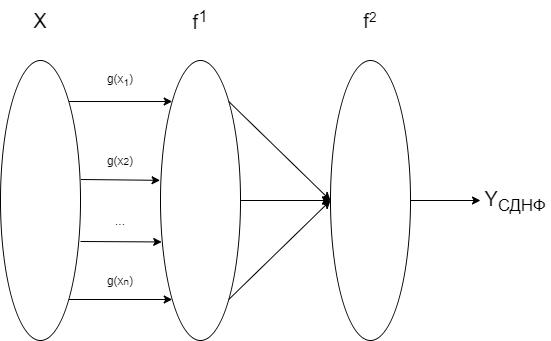
\includegraphics[width=1\linewidth]{picture1.png}
    \caption{}
    \label{ris:experimcoded}
    \end{center}
    \end{figure}
    
    Так как СДНФ функции конечна и единственна, то по ней мы сможем однозначно восстановить все функции алгебры логики, и такая нейронная сеть будет полна, что и требовалось доказать.
    \end{proof}
    
    Исторически, проблема выразимости нейронных сетей с вещественными значениями прослеживается от 13-й проблемы Гильберта, ставящей вопрос "существует ли непрерывная функция трех переменных, которая не может быть представлена через композицию непрерывных функций двух переменных". Она была решена в 1957 г. В.А. Арнольдом; oн показал, что любая непрерывная функция трех переменных представляется в виде композиции непрерывных функций двух переменных. В том же 1957 г. А.Н. Колмогоров доказал более сильную теорему: для реализации функций многих переменных достаточно операций суммирования и композиции функций одной переменной. Эта теорема в 1987 году была переложена Хехт–Нильсеном для нейронных сетей: любая функция нескольких переменных может быть представлена двухслойной нейронной сетью с прямыми полными связями с $N$ нейронами входного слоя, $(2N+1)$ нейронами скрытого слоя с ограниченными  функциями активации (например, сигмоидальными) и $M$ нейронами выходного слоя с неизвестными функциями активации \cite{seventh, eighth, ninth, tenth}.
    
    В бинарных нейронных сетях класса $\mathfrak{B}$ справедлив аналогичный результат.
    
    \begin{theorem}
    Какое бы семейство функций активации $F$ мы не взяли, класс бинарных нейронных сетей $\mathfrak{B}$ с четырьмя слоями будет полон в $P_2$.
    \end{theorem}
    
    \begin{proof}
    Из доказательства критерия Поста \cite{eleventh} известно, что имея нелинейную функцию, инвертор и константу 1, получим конъюнкцию. Имея конъюнкцию и инвертор, получим дизъюнкцию. Такая система будет полна. Среди линейных функций есть константа 1 и инвертор, в роли которого будет выступать исключающее «или» в виде $\overline{x} = 1 \oplus x$. Тогда на первом слое мы получим конъюнкцию, на втором — дизъюнкцию, а на третьем и четвертом — мы построим СДНФ нужной функции по \textbf{Теореме 2}.
    \end{proof}
    
    
\subsection{Аппроксимация}   
    В практике расчетов, связанных с обработкой экспериментальных данных, вычислением $f(x)$, разработкой вычислительных методов, встречаются следующие две ситуации:
    
    \begin{enumerate}
    \item Как установить вид функции $y = f(x)$, если она неизвестна? Предполагается при этом, что задана таблица ее значений, которая получена либо из экспериментальных измерений, либо из сложных расчетов.
    \item Как упростить вычисление известной функции $f(x)$ или же её характеристик, если $f(x)$ слишком сложная?
    \end{enumerate}
    
    Ответы на эти вопросы даются теорией аппроксимации функций, основная задача которой состоит в нахождении функции $\varphi(x)$, близкой (т.е. аппроксимирующей) в некотором нормированном пространстве к исходной функции $y = f(x)$. Функцию $\varphi(x)$ при этом выбирают такой, чтобы она была максимально удобной для последующих расчетов.
    
    Одним из замечательных свойств нейронных сетей с вещественными значениями является способность аппроксимировать и, более того, быть универсальными аппроксиматорами. С их помощью можно аппроксимировать сколь угодно точно непрерывные функции многих переменных. \cite{twelfth}
    
    Что касается бинарных нейронных сетей, здесь этот вопрос ещё хорошо не изучен. Важно доказать, насколько хорошо можно аппроксимировать любую булеву функцию линейными, то есть важен вопрос линейной аппроксимации в бинарном случае.
    
    \begin{definition}
    Пусть $f$ — булева функция от $n$ переменных, то есть $f: V^n \rightarrow \{0, 1\}$, где $V^n$ "--- булевый вектор размерности $n$. Ее \emph{весом} $w(f)$ будем называть количество наборов, на которых функция принимает значение 1.
    \end{definition}
    
    \begin{definition}
    Пусть $f, g$ — булевы функции от $n$ переменных. \emph{Расстоянием} от булевой функции $f$ до булевой функции $g$ называется величина $$dist(f, g) = w(f \oplus g),$$ то есть количество наборов, на которых значения $f$ и $g$ различаются. Расстоянием от $f$ до множества $M$ булевых функций от $n$ переменных назовем величину $$dist(f, M) = \min_{g \in M}\ dist(f, g).$$
    \end{definition}
    
    %Скажем, что булева функция $f$ \emph{близка} к булевой функции $g$, если расстояние $dist(f, g)$ между ними меньше некоторого фиксированного числа $\varepsilon$. В противном случае скажем, что булева функция $f$ \emph{далека} от булевой функции $g$. Аналогично и для расстояния между функцией $f$ и множества $M$.
    
    \textbf{Гипотеза.}
    Всегда найдется булева функция $f$ из класса нелинейных функций такая, что расстояние от нее до класса линейных будет больше числа $k \in \mathbb {N}$, то есть $dist(f, L) > k$.
    
    \textbf{Задача.}
    Найти максимальное число $k$, при котором гипотеза будет верна.
    
    \emph{Основная идея.}
    Известно, что линейных булевых функций от $n$ переменных $2^{n+1}$, а нелинейных "--- $2^{2^n} - 2^{n+1}$. То есть при $n \geqslant 3$ количество нелинейных функций начинает преобладать над количеством линейных.
    Необходимо рассмотреть систему шаров радиусами $k$, центрами которых будут линейные функциии. Внутри этих шаров будут нелинейные функции. Начиная с $k = 1$, увеличивать значение радиусов шаров на 1, пока все нелинейные функции не попадут в них. Итоговый радиус и будет порогом, когда линейные функции получают способность аппроксимировать нелинейные.
    
    Получив значение $k$, мы определим, насколько далеки нелинейные булевы функции от линейных. 
\newpage

\section{Заключение}
    В данной работе исследована проблема полноты бинарной нейронной сети. Доказывается, что для полноты бинарных нейронных сетей, слоем которой является композиция линейной булевой функции и нелинейного бинарного оператора, в некоторых случаях достаточно двух слоев, а  в общем случае "--- четырёх. В дальнейшем планируется получить результаты по глубине для разных функций активации.
    
    Обозначена важность проблемы аппроксимации булевых функций линейными функциями.
    Предложена идея доказательства плохой аппроксимации линейными функциями. Ставится цель изучить аппроксимацию в бинарном случае нейронной сетью, в слое которой будут линейные функции и некоторые нелинейности, а также применять подобную архитектуру в практических задачах.
    
    Автор выражает благодарность И. Е. Иванову за научное руководство.
\newpage

\begin{thebibliography}{99}

\bibitem{first} Courbariaux, M.; Bengio, Y. BinaryNet: Training Deep Neural Networks with Weights and Activations Constrained to $+1$ or $-1$. arXiv:1602.02830.
    
\bibitem{second} Rastegari, M.; Ordonez, V.; Redmon, J.; Farhadi, A. XNOR-Net: ImageNet Classification Using Binary Convolutional Neural Networks. In Proceedings of the European Conference on Computer Vision, Amsterdam, The Netherlands, 11–14 October 2016; pp. 525–542.32.
    
\bibitem{third} Zhou, S.; Ni, Z.; Zhou, X.; Wen, H.; Wu, Y.; Zou, Y. DoReFa-Net: Training Low Bitwidth Convolutional Neural Networks with Low Bitwidth Gradients. arXiv 2016, arXiv:1606.06160.
    
\bibitem{fourth} Tang, W.; Hua, G.; Wang, L. How to Train a Compact Binary Neural Network with High Accuracy? In Proceedings of the Thirty-First AAAI Conference on Artificial Intelligence, San Francisco, CA, USA, 4–9 February 2017
    
\bibitem{fifth} Darabi, S.; Belbahri, M.; Partovi Nia, V.; Courbariaux, M. Regularized Binary Network Training. arXiv:1812.11800
    
\bibitem{sixth} Simons, T.; Lee, D. A Review of Binarized Neural Networks. Electrical and Computer Engineering, Brigham Young University, Provo, UT 84602, USA.
    
\bibitem{seventh} Колмогоров А. Н. О представлении непрерывных функций нескольких переменных суперпозициями непрерывных функций меньшего числа переменных. ДАН СССР, 1956, Т.108, №2, С. 179-182
    
\bibitem{eighth} Арнольд В.И. О функции трех переменных. ДАН СССР, 1957, Т.114, №4, С. 679-681
    
\bibitem{ninth} Колмогоров А. Н. О представлении непрерывных функций нескольких переменных в виде суперпозиций непрерывных функций одного переменного и сложения. ДАН СССР, 1957, Т.114, №5, С. 953-956
    
\bibitem{tenth} Hecht-Nielsen R. Kolmogorov’s mapping neural network existence theorem. IEEE First Annual Int. Conf. on Neural Networks, San Diego, 1987. Vol. 3. — P. 11—13.

\bibitem{eleventh} Алексеев В. Б. Дискретная математика (II семестр). — М., МГУ, 2002. — 44 с.

\bibitem{twelfth} Cybenko, G. V. Approximation by Superpositions of a Sigmoidal function // Mathematics of Control Signals and Systems. — 1989. — Т. 2, № 4. — С. 303—314.

\end{thebibliography}
    
\end{document}